\chapter{Analyse \& Design ( 25 \%)}
\label{chap:design}


Im vorhergehenden Kapitel wurden Ziele und Leistungskriterien f\"ur das CI-System festgelegt.
Diese sollen nun auf konzeptueller Ebene umgesetzt werden.
Dazu wird zuerst ein \"Uberblick des Gesammtkonzeptes gegeben.
Anschliessend werden Besondere Konzepte zur 
%XXX: continue


\section{Grundlegende Systemarchitektur}
\label{sec:design:sysarch}
Diese Sektion gibt Aufschluss \"uber die Grobstruktuer des CI Systemes auf logischer und physischer Ebene.

\subsection{logisch}

\begin{figure}[ht]
  \centering
  \label{fig:grob-layout-komponenten-logisch}
  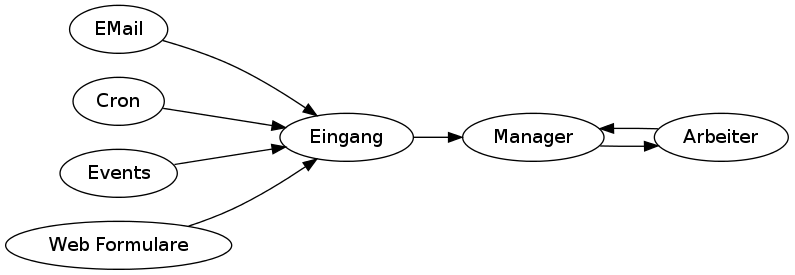
\includegraphics[width=\textwidth]{imageinput/grob-layout-komponenten-logisch.png}
  \caption{\"Ubersicht ber Systemkomponenten - logisch}
\end{figure}


Die erste wichtige Komponente ist der Eingang,
in ihm gehen Auftr\"age aus verschiedensten Quellen ein.
Nach dem sie validiert wurden, werden die Auftr\"age an
die zweite wichtige Komponente, den Manager, weitergegeben.
Dort werden sie vorbereitet und entsprechend der Build-Matrix Arbeitspackete erstellt.
Nun treten Manager und Arbeiter in eine Interaktion,
um zu bestimmen welcher Arbeiter das Eigentliche Arbeitspacket bearbeitet.
Anschliessend werden die Arbeitspackete von den jeweilig designierten Arbeitern abgefertigt.

%XXX: more


\subsection{physisch}

\begin{figure}[ht] 
  \centering
  \label{fig:grob-layout-komponenten}
  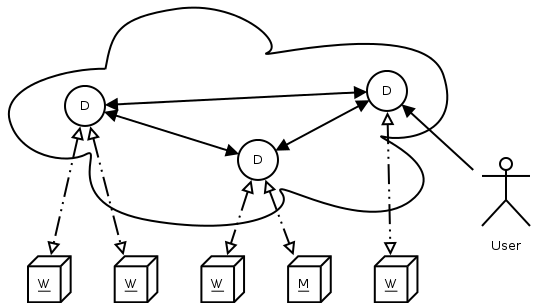
\includegraphics[width=\textwidth]{imageinput/grob-layout-komponenten.png}
  \caption{\"Ubersicht \"uber Systemkomponenten - physisch}
\end{figure}

Der physische Aufbau unterscheidet sich stark von den bisher dagewesenen CI-Systemen.
Grund ist der Focus auf die verteilte Datenbank, direkte Kommunikation
wird der Interaktion mit einer verteilten Datenbank weichen.

Das System besteht somit aus Komponenten welche alle als Clients einer verteilten Datenbank operieren.
Die Abbildung~\ref{fig:grob-layout-komponenten} zweigt die Struktur.
Nennenswert ist dabei die Bindung einer Komponente and bestimmte Datenbankknoten,
dies dient der Kontrolle der Lokalit\"at und wird sp\"ater noch vorgestellte Verfahrensweisen unterst\"utzen.

%XXX more

\section{Grundlegendes Datenschema}


\begin{figure}[ht] 
  \centering
  \label{fig:datenstrukturen}
  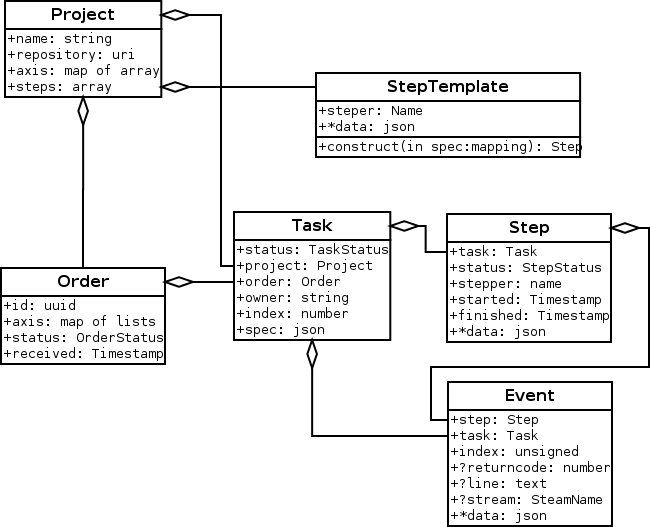
\includegraphics[width=\textwidth]{imageinput/datenstrukturen-step-templates.png}
  \caption{Grundlegende Datenstrukturen}
\end{figure}

Das grundlegende Datenschema, in Abbildung~\ref{fig:datenstrukturen} als UML Klassendiagramm dargestellt,
beschreibt die Daten des Kernsystemes und einige ihrer Interaktionen.

Die wichtigsten Datentypen sind dabei Projekt, Auftrag (Order), Arbeitspacket (Task) und Arbeisschritt (Step).

\subsubsection{Projekt}

Das Projekt beinhaltet neben dem Namen auch alle Informationen,
die sp\"ater f\"ur das erstellen von Arbeitspacketen sowie
das ausf\"uhren einer Integration ben\"otigt werden.
Dazu geh\"ort das Quellcode-repository (repo), von dem sp\"ater
die Quelltexte f\"ur das dem Test unterworfenen bezogen werden.
Weiterhin beinhaltet es die Build-Achsen,
welche die Wertebereiche der einzelnen Ebenen der Build-Matrix
beschreiben.

\subsubsection{Arbeitsschritt Template}

Der Mitunter wichtigste Teil eines Projektes ist jedoch die Beschreibung der Arbeitsschritte als Templates.
Die Darstellung als Template ist dabei bewusst gew\"ahlt,
sie erm\"oglicht es jedem Arbeitspacket speziell konfigurierte Arbeitsschritte zur Verf\"ugung zu stellen.
Ausserdem bewirkt die erneute Speicherung als neue Datenbankobjekte,
das Bearbeiten der Schritte eines Projektes keinen Einfluss auf bereits erstellte Arbeitspackete hat.
Zudem stellen die extra Objekte auch einen Anschlusspunk f\"ur die Datensammlung dar.
Die Methode \textit{construct} des Templates dient dazu,
einen Arbeitsschritt, angereichert mit einer entsprechenden Konfiguration, zur\"uckzugeben.

\subsubsection{Auftrag}

Ein Auftrag beinhaltet grunds\"atzlich eine Referenz auf das zugeh\"orige Projekt,
ausserdem beinhaltet er \"Uberschreibungen/Zus\"atze f\"ur die Build-Achsen,
dies Erm\"oglicht es sowohl in den Achsen eingeschr\"ankte, als auch erweierte Auftrage zu erstellen.
Diese werden sp\"ater genauer erkl\"art.
Zus\"atzlich beinhaltet der Auftrag einen Status, dieser beinhalted den aktuellen Stand der Bearbeitung.

\subsubsection{Arbeitspacket}
%XXX: eventuell projekt hier nicht referenzieren
Ein Arbeitspacket beinhaltet neben Referenzen zu dem Projekt und dem Auftrag,
seine Spezifikation. Diese gibt die Ausbildung aller Build-Achsen f\"ur dieses Packet an.
des weiteren beinhaltet es den Index, dieser gibt die Numerische Position in der Build-Matrix an.
Auch ein Arbeitspacket hat einen Status, welcher den aktuellen Bearbeitungstand zum Ausdruck bringt.
Zudem bestimmt das Feld ``Owner'' den Arbeiter, welcher das Arbeitspacket letztendlich bearbeiten wird.

\subsubsection{Arbeitsschritt}

Ein Arbeitsschritt referenziert das zugeh\"orige Arbeitspacket.
Neben den Zeitpunkten f\"ur Anfang und Ende seiner Ausf\"ugrung,
bennennt er im Feld ``stepper'' um welche Art von Arbeitsschritt es sich handelt.
Das Feld ``status'' gibt Auskunft \"uber den aktuellen Bearbeitungsstand.
Das Feld ``data'' soll weitere dynamische Informationen zum Ausdruck bringen,
die bei der Ausf\"uhrung genutzt werden.

%XXX: dies dient \ldots


\subsubsection{Event}
%XXX referenz auf task?

Das Event bringt Datensammlung zur Laufzeit zum Ausdruck.
Neben den Referenzen f\"ur den Arbeitschritt und das Arbeitspacket,
beinhaltet es die Indexnummer und einen Timestamp.
Die Indexnummer ist eine aufsteigende Zahl
und gibt den Events eines bestimmten Arbeitsschrittes eine feste eindeutige Reihenfolge.
Der Timestamp gibt den Events eine zeitliche Ordnung (welche jedoch nicht eindeutig ist).


Zus\"atzlich zu diesen Basisdaten, beinhaltet ein Event beliebige weitere optionale Felder.
Einige m\"ogliche (und ihre Datentypen) sind:

\begin{description}
    \dhitem[returncode: Number] R\"uckgabewert eines Prozesses bei seiner Beendigung.
    \dhitem[line: Text] Textzeile eines Ausgabestromes
    \dhitem[lineno: Number] Zugeh. Zeilennummer
    \dhitem[stream: Name] Zugeh. Name des Ausgabestromes
    \dhitem[start: Name] Mitteilung \"uber den Start eines best. Vorganges
    \dhitem[end: Name] Mitteilung \"uber den Abschluss eines best. Vorganges
\end{description}




\section{Grundlegende Logik der Komponenten}

Siese Sektion behandelt die grundlegende Logik %XXX MORE

\subsection{Auftragsannahme}

Der Auftragsannahme l\"asst sich grob in 2 Abschnitte einteilen.
Zuerst geht ein Aufrag ein, was je nach Methode in mehrere Schritte beinhalten knann,
dannach wurd er \"uberpr\"uft und damit angenommen oder abgelehnt.


\begin{figure}[ht]
  \centering
  \label{fig:lebenszyklus-auftrag-eingang}
  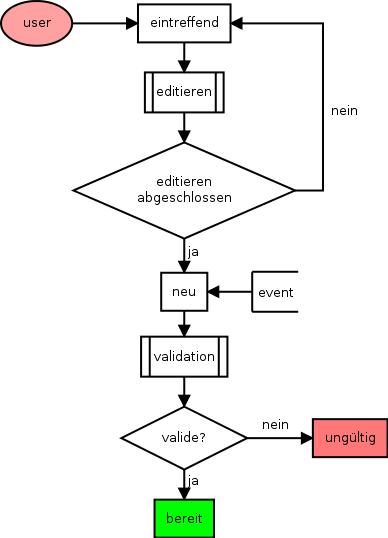
\includegraphics[height=5in]{imageinput/lebenszyklus-auftrag-eingang.png}
  \caption{Auftragsannahme: Flowgraph}
\end{figure}


\subsubsection{Eingang}

Auftragseingang gestaltet sich in der Praxis vielseitig.
Da nicht alle Quellen direkt einen fertigen Auftrag generieren k\"onnen,
beginnt ein Auftrag im Zustand eingehend, sind schliesslich alle Daten zusammengekommen,
so wird der Eingang festgehalten und der Auftrag wird vom System weiterverarbeitet.

%XXX Quellen betrachten``


\begin{verbatim}
- quellen
- editiern
- typisches
-> eine auswaehlen
\end{verbatim}

\subsubsection{Validation}

%XXX: genauer beschreiben

Die Validation verfolgt das Ziel, Auftr\"age auch aus weniger vertrauensw\"urdigen Quellen anzunehmen.
Dies erm\"oglicht Verwendung \"ahnlich zu TravisCI, was es erlaubt, Zuarbeiten von Aussenstehenden zu Testen.
F\"ur die \"Uberpr\"ufung stehen verschiedene M\"oglichkeiten zur Verf\"ugung.
Ein Eingang per Email/Malingliste oder Pull-Request auf einer Code-Hosting,
kann z.b. nach erstmaliger Erlaubniss, wiederholt zugelassen werden,
w\"ahrend Informationen die Mitarbeiter einsenden z.b. an ihr Arbetsverh\"altniss gebunden werden k\"onnen.

Zeitgesteuerte Eing\"ange innerhalb des Systemes k\"onnen jedoch grunds\"atzlich zugelassen werden.

Den Abschluss der Validation stellt die Markierung des Auftrages als Valide oder invalide dar.

\subsection{Management}

\begin{figure}[ht] 
  \centering
  \label{fig:lebenszyklus-auftrag-abarbeitung}
  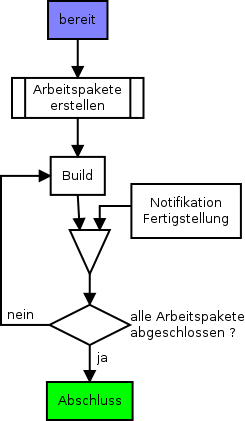
\includegraphics[height=4in]{imageinput/lebenszyklus-auftrag-abarbeitung.png}
  \caption{Auftragsannahme: Flowgraph}
\end{figure}

\subsubsection{Auftragsvorbereitung}

In der Auftragsvorbereitung werden Managementdaten zum Auftrag hinzugef\"ugt.
Die vordefinierten Build-Achsen werden vom Projekt \"ubertragen.
Dies stell sicher, dass der Aufrag und sein Umfang eindeutig bestimmt sind,


\subsubsection{Bereitstellung von Arbeitspacketen}

Das Bereitstellen von Arbeitspacketen stellt den Anfang der eigentliche Arbeitsphase dar.
Entsprechend der Werte der Build-Achsen des Auftrages, werden nun die Arbeitspackete generiert,
wobei jedes Arbeitspacket eine der Wertekombinationen darstellt.
Nachdem alle Arbeitspackete erstellt sind, ist die Bearbeitung des Auftrages an sich abgeschlossen.

\subsubsection{Abschluss von Auftr\"agen}

Der Abschluss eines Auftrages ist ein Ereigniss welches Impliziert werden kann.
In dieser Arbeit wird der Abschluss eines Auftrages definert als der Zustand der Eintritt,
wenn alle Arbeitspackete eines Auftrages einen finalen Zustand erreichen.

Dies Vereinfacht die Behandung des Auftragsabschlusses,
da man nicht nach Abschluss von Arbeitspacketen weitere Operationen durchf\"uhren muss,
um den eventuellen Abschluss festzustellen.

\subsection{Zuteilung/Abarbeitung von Arbeitspacketen}


\subsubsection{Lebenszyklus eines Arbeitspacketes}


\begin{figure}[ht] 
  \centering
  \label{fig:lebenszyklus-arbeitspaket}
  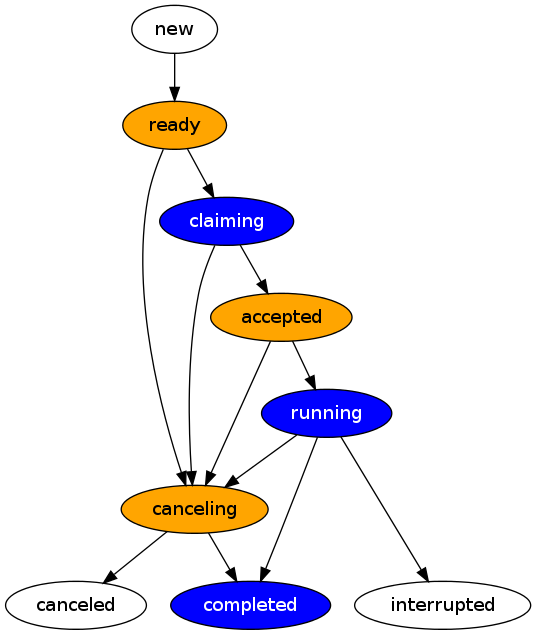
\includegraphics[height=4.5in]{imageinput/lebenszyklus-arbeitspaket.png}
  \caption{Lebenszyklus eines Arbeitspacketes bei Ausschreibungen}
\end{figure}


\subsubsection{Vorbereitung Abarbeitung}

\subsection{\"Uberblick Zuteilungsmethoden}


\begin{verbatim}
- diese sektion besch. sich mit


- methoden
    - token basiert
    - ausschreibungsbasiert

\end{verbatim}


\subsubsection{token basierte zuweisung}

\begin{verbatim}
- arbeiter teilen nur mit, dass sie arbeitsfaehig sind
- manager kontrolliert wer welchen auftrag erhaelt
cons:
    - fuer erweiterte use-cases extra wissen im manager notwendig
\end{verbatim}

\begin{figure}[ht] 
  \label{fig:auftrag-zuteilung-token}
  \begin{sequencediagram}
      \newinst{worker}{:Worker}
      \newinst[1]{manager}{:Manager}
      \mess{worker}{token <spec>}{manager}
      \mess{manager}{work <spec>}{worker}
      \mess{worker}{result}{manager}
  \end{sequencediagram}
  \caption{Auftragszuteilung: Tokenbasiert}
\end{figure}

\subsubsection{ausschreibungsbasierte zuweisung}

\begin{verbatim}
- manager teilt offene auftraegeposten mit (in datenbank verf.)
- arbeiter konkurieren um offene auftraege
- manager entscheidet wer den aufrag dann erhaelt


- autonomere arbeiter
- manager muss nur noch entscheiden wer, nicht mehr warum
- aufgrund der datenbank konzeptuell einfacher -> beweis oder weg
\end{verbatim}

\begin{figure}[ht] 
  \label{fig:auftrag-zuteilung-claim}
  \begin{sequencediagram}
      \newinst{workera}{:Worker A}
      \newinst[1]{manager}{:Manager}
      \newinst[1]{workerb}{:Worker B}
      \mess[1]{manager}{availiable}{workera}
      \prelevel
      \prelevel
      \mess[1]{manager}{availiable}{workerb}

      \mess[1]{workera}{claim}{manager}
      \prelevel
      \prelevel
      \mess[2]{workerb}{claim}{manager}
      %XXX: better call?
      %\prelevel
      %\prelevel
      %\begin{call}{manager}{approve}{manager}{workera}
      %\end{call}
      \mess{manager}{approve A}{workera}
      \prelevel
      \mess{manager}{approve A}{workerb}
  \end{sequencediagram}
  \caption{Auftragszuteilung: Ausschreibungsbasiert}
\end{figure}


\subsubsection{Abschluss Abarbeitung}

- ende der arbeisschritte
- zusammenfassung resultat
- endscheidung fehlschlag oder nucht


\subsection{Abarbeitung von Arbeitspacketen}

\begin{verbatim}
- lineare abarbeitung
- abbrich bei fehlschlag
\end{verbatim}

\subsubsection{Arbeitsschritte}


\begin{figure}[ht] 
  \centering
  \label{fig:lebenszyklus-arbeitsschritt}
  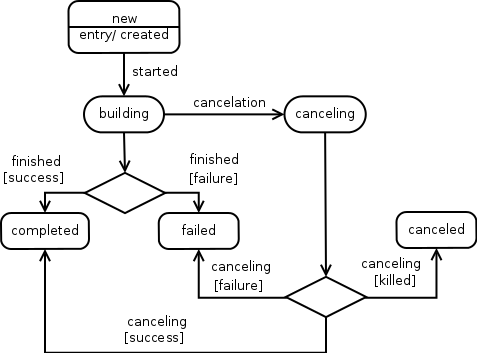
\includegraphics[height=3.4in]{imageinput/lebenszyklus-arbeitsschritt.png}
  \caption{Stategraph eines Arbeitschrittes}
\end{figure}

\begin{verbatim}
- kill wird in der impl nicht betrachtet

\end{verbatim}


\subsubsection{Datensammlung zur Laufzeit}

\begin{verbatim}
- sinn/echtzeit?

- beispielhaft
    - STDOUT/ERR
    - exakte testresultate/reports
\end{verbatim}

\subsubsection{Datensammling nach Abschluss eines Schrittes}

- junitxml
- logfiles

- betrachtung extra schritt vs interne funktion

\subsubsection{Abschluss von Arbeitschritten}

- returncodes
- fehler

\subsection{Arten von Arbeitschritten}

\subsubsection{\"Ubersicht}

\begin{figure}[h!]
  \centering
  \label{fig:klassen-arten-arbeitsschritt}
  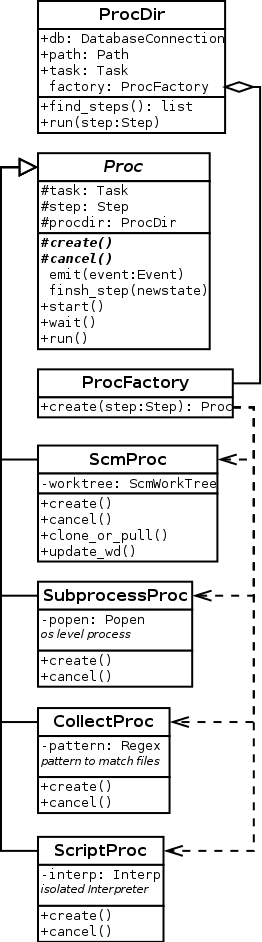
\includegraphics[height=3.5in]{imageinput/klassen-arten-arbeitsschritt.png}
  \caption{Arten von Arbeitschritten}
\end{figure}


\FloatBarrier
\subsubsection{Prozessaktionen}

- was/wozu
- datensammlung laufzeit
- datensammlung ende

\subsubsection{Quellcode Management Aktionen}

- ablauf, beispiele



\section{Besondere Ans\"atze zur Datenbankinteraktion}

%XXX: http://dbmsmusings.blogspot.de/2010/04/problems-with-cap-and-yahoos-little.html


\subsection{CAP Abdeckung}

Wie bereits in Sektion~\ref{sec:base:cap} erw\"ahnt,
ist es immer nur m\"oglich 2 der 3 Aspekte des CAP Theorems abzudecken.

Jedoch ist es durchaus legitim f\"ur verschiedene Teile einer Applikation unterschiedliche Bereiche abzudecken.
Sobald genau definiert ist, f\"ur welche Daten in welchem Kontext welche Eigenschafen benoetigt werden,
kann ein konsistentes Modell geschaffen werden.

Wichtig ist bei dieser Betrachtung, dass die Unterschiedlichen des Entwickelten CI-Systemes
nicht zwingend eine direkte Konsistenzbindung untereinander ben\"otigen.
Wichtig ist nur, die Konsistenz zwischen einer Komponente und dem Datenbankknoten,
mit dem sie Kommuniziert.

Das Hauptsystem, in dem alle Komponenten in Kommunikation stehen,
%XXX: s1?
soll nach Systemanforderung \textbf{S1} immer verf\"ugbar sein, und Teilausf\"alle verkraften.
Somit kommt f\"ur die Kommunikation zwischen Komponenten nur das Model \textbf{A-P} in Frage
(was Verf\"ugbar und Partitionstollerant bedeutet).

Die Anbinding einzelner Komponenten and ihre Datenbankknoten, hat jedoch andere Anforderungen.
Da eie direkte Anbindung and die Datenbank f\"ur das Funktionieren einer Komponente unabdingbar ist,
kann in diesem Fall nur das Modell \textbf{C-A} zum Einsatz kommen.


%XXX: http://www.infoq.com/articles/cap-twelve-years-later-how-the-rules-have-changed


\subsection{Statusmaschienen zur Konsistenzwahrung}

%XXX: Literatur
% http://blog.incubaid.com/2012/10/25/caulking-your-distributed-algorithm-implementation/
\nocite{statechart}

Statusmaschienen sind ein allgemein bekanntes Werkzeug,
um den den Ablauf eines komplexen Programmes zu beschreiben oder zu erkl\"aren.
In der Regel wird dazu ein sog. StatusGraph verwendet.
Dieser ist ein Gerichteter Graph der die Zust\"ande und Zustands\"anderungen eines Systemes beschreibt.

Wie bereits in Abbildung \ref{fig:lebenszyklus-arbeitspaket} gezeigt,
stellt der Lebenszyklus eines Arbeitspacketes einen solchen Statusgraph dar.
Als Besonderheit ist er sogar frei von Zyklen.
Dadurch ist es unm\"oglich den gleichen Status noch einmal zu erreichen.

Bindet man Zus\"atzlich noch die Transitionen an bearbeitende Knoten (Agenten ausserhalb der Datenbank),
so ist es auch bei einer Partitionierung der Datenbank eine Konsistenz der Gesammtsystemes gew\"ahrleistet.

%XXX: moar?


Mit dem dem Eingang und der Abarbeitung von Auftr\"agen verh\"alt es sich \"ahnlich,
jedoch ist der Graph dort Wesentlich einfacher.
Die Abbildungen \ref{fig:lebenszyklus-auftrag-eingang} und \ref{fig:lebenszyklus-auftrag-abarbeitung} zeigen den groben Ablauf.
Der Wechselpunkt zwischen Eingang und Abarbeitung ist die der Validation angeschlossene Markierung zur Bereitschaft.
Da es nur diesen einen Punkt des Austausches gibt, ist die Konsistenzwahrung des Auftrages Denkbar einfach,
Mit der Bereitschaft, wird die Verwantwortung vom Eingang zur Abarbeitung \"ubertragen.


\section{auftragsverteilung}

\section{Logisches Gesammtkonzept}


\section{Arbeitsschritte}

\section{Benutzerinterface}

% kann krit
% kein tolles
% nur werkzeuge


\section{zusammenfassung}

was kommt
was kommt nicht
